%*****************************************
\chapter{Phonetic-based Speller}\label{ch:speller}
%*****************************************

\section*{Abstract}
\footnote{This chapter contains an extended version of the recently submitted paper: \bibentry{Mendonca2015}}
Recently, spell checking (or spelling correction systems) has regained attention 
due to the need of normalizing user-generated content (UGC) on the web. UGC presents 
new challenges to spellers, as its register is much more informal and contains much
more variability than traditional spelling correction systems can handle. This chapter proposes 
two new approaches to deal with spelling correction of UGC in Brazilian Portuguese (BP), 
both of which take into account phonetic errors. The first approach is based on three phonetic
modules running in a pipeline. The second one is based on machine learning, with soft decision 
making, and considers context-sensitive misspellings. We compared our methods with 
others on a human annotated UGC corpus of reviews of products. The machine learning approach surpassed 
all other methods, with 78.0\% correction rate, very low false positive (0.7\%) and false 
negative rate (21.9\%). 

\section{Introduction}

Spell checking is a very well-known and studied task of natural language processing (NLP), being present in applications used by the general public, including word processors and search engines. Most of the methods of spell checking are based on large dictionaries to detect non-words, mainly related to typographic errors caused by key adjacency or fast key stroking. 
%Such kind of error was the basis of the first spell checkers, dating back to Damerau \cite{Damerau1964}, which addressed the problem by analyzing the edit distance of the words. 
Currently, with the recent boom of mobile devices, with small touchscreens and tiny keyboards, one can miss the keystrokes, hitting adjacent keys on the keyboard, thus spell checking has regained attention \cite{Duan2011}.   

Dictionary-based approaches can be ineffective when the task is to detect and correct spelling mistakes which coincidentally correspond to an existing word (real-word errors). Different from non-word errors, real-word errors are context dependent. Several approaches have been proposed to deal with these errors: mixed trigram models \cite{Fossati2007}, confusion sets \cite{Fossati2008}, improvements on the trigram-based noisy-channel model \cite{Mays1991} and \cite{WilcoxOHearn2008}, use of GoogleWeb 1T 3-gram data set and a normalized and modified version of the Longest Common Subsequence string matching algorithm \cite{Islam2009}, a graph-based method using contextual and PoS features and the double metaphone algorithm to represent phonetic similarity \cite{Sonmez2014}. As an example, although MS Word (from 2007 version to on) claims to include a contextual spelling checker, an independent evaluation of it found high precision but low recall in a sample of 1400 errors \cite{Hirst2008}.

Errors due to phonetic similarity also impose difficulties to spell checkers. They occur when a writer knows well the pronunciation of a word but does not know how to spell it. This kind of error requires new approaches to combine phonetic models and models for correcting typographic and/or real-word errors. In \cite{Zampieri2014}, for example, the authors use a linear combination of two measures -- the Levenshtein distance between
two strings and the Levenshtein distance between the Soundex \cite{soundex} code of two strings.
Phonetic errors usually occur due to inconsistent spellings rules, ambiguous word breaking and fast introduction of new words, mainly related to technology jargon, affecting both native and non-native speakers of a language \cite{Duan2011}. 

\cite{Baptista2011} detail these problems in a typology of spelling errors in the scenery of written language acquisition: errors produced by lack of understanding of  letter-to-sound correspondences in written language, by fails in the transcription of the oral language, by breaking rules based on phonology or morphology and by inconsistent spelling rules. Due to these several kinds of error this task is still difficult.

Some applications require interactive spelling correction (e.g. typing a text or a search query),  whereas others require fully automatic correction, (e.g. corpus normalization). While in the first kind of applications the spell checker presents several suggestions to the user, the second one requires a spell checker that elects the better suggestion (first hit accuracy), as there is no user to take the decision.

In the last decade, some researchers have revisited spell checking issues motivated by web applications, such as search query engines and sentiment analysis tools based on natural language processing (NLP) of UGC, e.g. Twitter data or product reviews.
The search engine Google has turned popular the facility of auto-completing, where suggestions to prefixes of a query are offered; this is still a process of interactive spelling correction. There is also another kind of facility where a unique suggestion is given after the query is typed, with the link of the documents recovered for it \cite{Duan2011}, \cite{Cucerzan2004}. This facility demands a high precision automatic spelling correction. 

Normalization of UGC has received great attention also because the performance of NLP tools (e.g. taggers, parsers and named entity recognizers) is greatly decreased when applied to UGC. Besides misspelled words, this kind of text presents a long list of problems, such as acronyms and proper names with inconsistent capitalization, abbreviations introduced by chat-speak style, slang terms mimicking the spoken language, loanwords from English as technical jargon, as well as problems related to ungrammatical language and lack of punctuation \cite{Duran2014,DeClercq2013,Han2013,Andrade2012}.
UGC normalization also requires automatic spelling correction, i.e., there is a need to automatically select the word that will more likely correct the misspelled word, not relying on a list of candidates for human selection. 

In \cite{Andrade2012} the authors propose a spell checker for Brazilian Portuguese (BP) to work on the top of Web text collectors. They have tested their method on news portals and on informal texts collected from Twitter in BP. However, they do not inform the error correction rate of the system. Furthermore, while their focus is on the response time of the application, they do not address real-word errors.

This chapter presents two new spell checking methods for UGC in BP. The first of them deals with phonetically motivated errors, a recurrent problem in UGC not addressed by traditional spell checkers. The second one deals additionally with real-word errors.
We present a comparison of these methods with a baseline system and JaSpell over a new and large benchmark corpus for this task. The corpus contains product reviews with 38,128 tokens and 4,083 annotated errors. Such corpus is also a contribution of our study\footnote{The small benchmark of 120 tokens used in \cite{Martins2004} and \cite{Ahmed2009} 
is not representative of our scenario.}. 

This chapter is structured as follows. In Section~\ref{sec:speller-method} we describe our methods, the setup of the experiments and the corpus we compiled. In Section~\ref{sec:speller-results} we present the results. In Section~\ref{sec:speller-related} we discuss related work on spelling correction of phonetic and real-word errors. To conclude, the final remarks are outlined in Section~\ref{sec:speller-final-remarks}.

\section{Experimental Settings and Methods}\label{sec:speller-method}

In this Section we present the four methods compared in our evaluation. Two of them are used by existing spellers, one is taken as baseline and the other is taken as benchmark. The remaining two are novel methods developed within the project reported herein. After describing in detail the novel methods, we present the corpus specifically developed to evaluate BP spellers, as well as the evaluation metrics.
The first one is the open source spell checker JaSpell for Portuguese (Baseline method). The second is acombination of phonetic rules and Soundex applied to candidates generated by 1 and 2 edit distance (Benchmark method). The third (nome1) and the fourth (nome2) are the two novel methods presented by this paper. The (nome1) is an improvement of the Benchmark method, a pipeline of three phonetic modules applied to candidates generated by 1 and 2 edit distance and by phonetic similarity - a manually built set of phonetic-based rules, a grapheme-to-phoneme converter, and the Soundex method adapted to BP (called here as Grapheme-to-Phoneme method). The (nome2) is a context-sensitive speller, based on machine learning, applied to candidates generated by 1 and 2 edit distance, by phonetic similarity and by word combinations of diacritics (called here as Machine Learning).
 
If none of these phonetic modules succeed, the second layer chooses the best candidate according to its edit-distance (the lower, the better) and to its frequency in large BP corpus (the bigger, the better); 
In both methods (Grapheme-to-Phoneme and Rules\&Soundex), if none of the phonetic modules succeed, a second layer chooses the best candidate according to its edit-distance (the lower, the better) and to its frequency in large BP corpus (the bigger, the better).

The aim of our experiments is to evaluate the effectiveness in the correction of common misspellings in UGC in BP of different phonetic-based methods applied on a corpus of product reviews. In this research we do not focus on errors related to acronyms, proper names, abbreviations, internet slang, technical jargon or loanwords in English. Instead, our goal is to assess the methods with regard to  phonetic-motivated errors and a special group of real-word errors in UGC due to the absence of diacritics.

\subsection{Method I - Baseline}

We use as a baseline the open source Java Spelling Checking Package, JaSpell\footnote {http://jaspell.sourceforge.net/}. JaSpell can be  considered a strong baseline and it is  employed at the tumba! Portuguese Web search engine to support interactive spelling checking of user queries. 
JaSpell classifies the candidates for a misspelled word according to the word frequency in a large corpus together with other heuristics, such as keyboard proximity or phonetic keys, provided by the Double Metaphone algorithm \cite{2000double} for the English language. At the time this speller was developed there was no version of these rules for the Portuguese language\footnote{Currently, a BP version of the phonetic rules can be found at http://sourceforge.net/projects/metaphoneptbr/}. 

\subsection{Method II - Benchmark}

The method presented in \cite{Avanco2014} is taken as benchmark. It combines phonetic knowledge in the form of a set of rules and the algorithm Soundex. It was inspired by the analysis of errors of the same corpus of products' reviews \cite{Hartmann2014} that inspired our proposals. Furthermore, as such method aims to be used for normalizing web texts, it performs automatic spelling correction. 

To increase the accuracy of the first hit, this method relies in some ranking heuristics. The strategies developed by the authors consider the phonetic proximity between the input wrong word and the candidates to substitute it. If the typed word does not belong to the lexicon, a set of candidates is generated by applying one and two edit distances from the original word and the words in the lexicon. Then a set of phonetic rules for Brazilian Portuguese codifies letters and digraphs which have similar sounds in a specific code. If necessary, the next step performs the algorithm Soundex, slightly modified for BP. Finally, if none of these phonetic-based algorithms is able to suggest a correction, the candidate with the highest frequency in a reference corpus among the ones with the least edition-distance is suggested. The lexicon used is the Unitex-PB\footnote{http://www.nilc.icmc.usp.br/nilc/projects/unitex-pb/web/} and the frequency list was taken from Corpus Brasileiro\footnote{http://corpusbrasileiro.pucsp.br/cb/}. The pseudocode for the algorithm can be found in Algorithm~\ref{alg:pseudocode-method2}.

\begin{algorithm}
\scriptsize
\caption{Method II -- Benchmark}\label{alg:pseudocode-method2}
\begin{algorithmic}[1]
\Procedure{CorrectWord}{w}
\If {w in Unitex}
\State \Return w
\Else
\State $w\_trans \gets pt\_rules(w)$ \Comment{apply PT-Rules to word}
\State $w\_soundex \gets soundex(w)$ \Comment{get word Soundex code}
\State $sugs \gets lev(Unitex,2)$ \Comment{get words with edit dist. 1 or 2}
\State \emph{\textbf{Look for rule transcription match}}:
\For{sug in sugs}
\State $sug\_trans \gets pt\_rules(sug)$
\If {$w\_trans = sug\_trans$} 
\State \Return sug
\EndIf
\EndFor
\State \emph{\textbf{Look for Soundex code match}}:
\For{sug in sugs}
\State $sug\_soundex \gets soundex(sug)$
\If {$w\_soundex = sug\_soundex$} 
\State \Return sug
\EndIf
\EndFor    
\State \Return{most frequent suggestion} 
\EndIf
\EndProcedure
\end{algorithmic}
\end{algorithm}


\subsection{Method III - Grapheme-to-Phoneme based Method (GPM)}

By testing the benchmark method, we noticed that many of the wrong corrections were related to a gap between the application of phonetic rules and 
the Soundex module. The letter-to-sound rules were developed specially
for the spelling correction, therefore, they are very accurate for the task but have a low recall, since many words do not possess the misspelling patterns 
which they try to model. In contrast, the transcriptions generated by the adapted
Soundex algorithm are too broad and many phonetically different words are given the same code. For instance, the words "perto" (\emph{near}) and "forte" (\emph{strong}) are both
transcribed with the Soundex code ''1630'', in spite of being very distinct phonetically: 
"perto" corresponds to \textipa{['pEh.tU]}, and "forte" to \textipa{['fOh.tSI]}.

To fill this gap we propose the use of a general-purpose grapheme-to-phoneme converter to be executed prior to the Soundex module. We selected Aeiouado's grapheme-to-phoneme converter \cite{Mendonca2014} 
for this purpose, since it consists of the state of the art in grapheme-to-phoneme transcription for Brazilian Portuguese. 
Aeiouado employs a hybrid approach for converting graphemes into phonemes, based on both manual transcription rules and machine learning algorithms. The transcription task is carried out in two stages: i) words are submitted to a set of transcription rules, in which predictable graphemes (mostly consonants) are transcribed; ii) a decision tree classifier is used to predict the transcription of the remaining graphemes (mostly vowels). The method achieved an average F1-score of 0.98 regarding to phone transcription. 
Since the converter was developed primarily for text-to-speech and automatic speech recognition, its transcriptions are too much detailed for spelling correction purposes. Only few words share exactly the same phone sequence. Therefore, we had to broaden the transcription, by grouping the mid-high and mid-low vowels together, by deleting the difference between nasal and oral vowels, by considering the many rhotic sounds into a single one, etc.

The usage of the grapheme-to-phoneme converter is a bit different from a simple pipeline. According to Toutanova \cite{Toutanova2002}, phonetic-based errors usually need larger edit distances to be detected. For instance, the word "durex" (\emph{sellotape}) and one of its misspelled forms "dur\'equis" have an edit distance of 5 units, despite having very similar or equal phonetic forms: \textipa{[du'rEks]} $\sim$ \textipa{[du'rEkIs]}. Therefore, instead of simply increasing the edit distance, which would imply in having a larger number of candidates to filter, we decided to do the reverse process. We transcribed the Unitex-PB dictionary and stored it into a database, with the transcriptions as keys. Thus, in order to obtain words which are phonetic similar words, we transcribe the input word and look it up in the database. Considering the "dur\'equis" example, we would first transcribe it as \textipa{[du'rE.kIs]}, and then check if there are any words in the database with this transcription. In this case, it would return "durex", the expected form.

The only difference of GPM in comparison with Method II lies in the G2P transcription match, which takes place prior to Soundex. The pseudocode for the algorithm can be found in Algorithm~ \ref{alg:pseudocode-method3}. 

\begin{algorithm}
\scriptsize
\caption{Method III -- GPM}\label{alg:pseudocode-method3}
\begin{algorithmic}[1]
\Procedure{CorrectWord}{w}
\If {w in Unitex}
\State \Return w
\Else
\State $w\_trans \gets pt\_rules(w)$ \Comment{apply PT-Rules to word}
\State $w\_phono \gets g2p(w)$ \Comment{apply G2P converter to word}
\State $w\_soundex \gets soundex(w)$ \Comment{get word soundex code}
\State $sugs \gets lev(Unitex,2)$ \Comment{get words with edit dist. 1 or 2}
\State \emph{\textbf{Look for rule transcription match}}:
\For{sug in sugs}
\State $sug\_trans \gets pt\_rules(sug)$
\If {$w\_trans = sug\_trans$} 
\State \Return sug
\EndIf
\EndFor
\State \emph{\textbf{Look for G2P transcription match in the database}}:
\If {any word that match $w\_phono$} 
\State \Return word
\EndIf
\State \emph{\textbf{Look for soundex code match}}:
\For{sug in sugs}
\State $sug\_soundex \gets soundex(sug)$
\If {$w\_soundex = sug\_soundex$} 
\State \Return sug
\EndIf
\EndFor    
\State \Return{most frequent suggestion} 
\EndIf
\EndProcedure
\end{algorithmic}
\end{algorithm}

In spite of being better than the baseline because they tackle phonetic-motivated errors, Method II and GPM have a limitation: they do not correct real word errors. The following method is intended to overcome this shortcoming by using context information.

\subsection{Method IV -- GPM in a Machine Learning framework (GPM-ML)}

Method IV has the advantage of bringing together many approaches to spelling correction into a machine learning framework. The architecture of the method is described in Figure~\ref{fig:sys3-architecture}. 

\begin{figure}[h!]
  \centering
    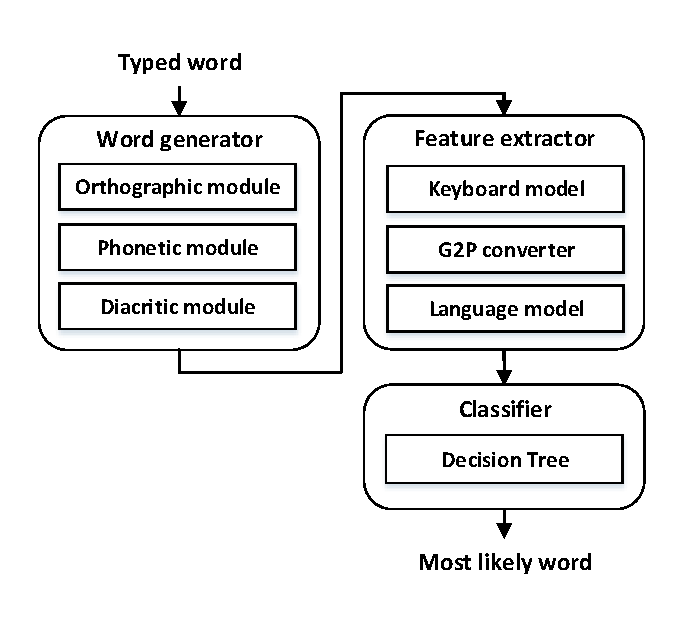
\includegraphics[width=0.7\textwidth]{gfx/speller_architecture.pdf}
\caption{\label{fig:sys3-architecture} \it Architecture of the GPM-ML}
\end{figure}
The method is based on three main steps: (i) candidate word generation, (ii) feature extraction and (iii) candidate selection. 
The word generation phase encompasses three modules which produce a large number of suggestions, considering the following aspects: orthographic, phonetic and diacritic similarities.
For producing suggestions which are typographically similar, the Levenshtein distance is used. For each input word, we select all words in a dictionary which diverge from the input by at most 2 units. For instance, suppose the user intended to write "mesa" (\emph{table}),  
but missed a keystroke and typed "meda" instead. The Levenshtein module would generate a number of suggestions including an edit distance of 1 or 2, such as "medo" (\emph{fear}), "meta" (\emph{goal}), "moda" (\emph{fashion}), "nada" (\emph{nothing}), "mexe" (\emph{he/she moves}) etc. For computational efficiency, we stored the dictionary in a trie structure, in order to make it quickly searchable. A revised version of the Unitex-PB was employed as our reference dictionary (\emph{circa} 550,000 words)\footnote{The dictionary is available upon request.}.

As for phonetic similarity, the Aeiouado's grapheme-to-phoneme converter \cite{Mendonca2014} was used to group phonetically related words. We transcribed the Unitex-PB word list  phonetically and stored all word transcriptions along with their orthographic form into a database, exactly as we did for GPM. Thus for generating suggestions which are phonetically similar to the word typed by the user, we obtain its phonetic transcription and look it up in the database.

The diacritic module is responsible for generating words which are similar to the word typed by the user with respect to diacritic symbols. This module was proposed since we observed that most of the misspellings in the corpus were caused by a lack or misuse of diacritics. BP has
five types of diacritics: accute (\'{}), cedilla (\c{c}), circumflex (\^{}), grave (\`{}) and tilde (\~{}). The diacritics often indicate different vowel quality, timbre or stress. However, these symbols are rarely used in UGC, and the reader uses the the context to  disambiguate the intended word. In order to allow the speller to deal with this problem, the diacritic model generates, given a word input, all possible word combinations of diacritics. Once more, the Unitex-PB is used as reference. 

After word generation, the feature extraction phase takes place. This phase is responsible  for extracting relevant information from the list of words generated in the previous step. The aim is to allow the classifier to compare these words with the one typed by the user, in such a way that the classifier is able to choose to keep the typed word or to replace it with one of the generated suggestions. 

As misspelling errors may be of different nature (such as typographical, phonological or related to diacritics), we try to select features that encompass all these phenomena. For each word suggestion produced in the word generation phase, we extract 14 features:

\begin{enumerate}
\setlength{\itemsep}{1pt}
\item \textsc{typedOrGen}: whether the word was typed by the user or was produced in the word generation phase;
\item \textsc{isTypo}: 1 if the word was generated by the typographical module; 0 otherwise;
\item \textsc{isPhone}: 1 if the word was generated by the phonetic module; 0 otherwise;
\item \textsc{isDiac}: 1 if the word was generated by the diacritic module; 0 otherwise;
\item \textsc{typedProb}: the unigram probability of the word typed;
\item \textsc{genUniProb}: the unigram probability of the word suggestion;
\item \textsc{typedTriProb}: the trigram probability of the word typed;
\item \textsc{genTriProb}: the trigram probability of the word suggestion;
\item \textsc{typoLevDist}: the levenshtein distance between the typed word and the suggestion;
\item \textsc{insKeyDist}: the sum of the key insertion distances;
\item \textsc{delKeyDist}: the sum of the key deletion distances;
\item \textsc{replKeyDist}: the sum of the key replacement distances;
\item \textsc{keyDists}: the sum of all previous three types of key distances;
\item \textsc{phoneLevDist}: the levenshtein distance between of the phonetic transcription of the typed word and of the suggestion. 
\end{enumerate}

The probabilities come from a language model trained over a subset of the Corpus Brasileiro (\emph{circa} 10 million tokens). Good-Turing smoothing is used to estimate the probability of unseen trigrams.
After feature extraction, the word selection phase comes into play. It consists of a Decision Tree Classifier which was trained over the dataset presented in Section~\ref{sec:dataset}, with the features we discussed. 
The classifier was implemented through scikit-learn \cite{Pedregosa2011} and comprises an optimized version of the CART algorithm. Several other classification algorithms were tested, but since our features contain both nominal and numerical data, and since some of them are dependent, the Decision Tree Classifier achieved the best performance.

\subsection{Dataset}\label{sec:dataset}

The evaluation corpus was compiled specially for this research and is composed of a set of  annotated product reviews, written by users on Buscap\'e\footnote{http://www.buscape.com.br/}, a Brazilian price comparison search engine. All misspelled words were marked, the correct expected form was suggested and the misspelling category was indicated.

We used snowball sampling to obtain a reasonable amount of data with incorrect orthography. A  list of ortographical errors with frequency greater than 3 in the  the corpus of product reviews compiled by \cite{Hartmann2014}
gathered by Avan\c{c}o ~\cite{Avanco2014} 
was used to pre-select, from the same corpus, sentences with at least
one incorrect word. Among those, 1,699 sentences were randomly
selected to compose the corpus (38,128 tokens). All these sentences
were annotated by two linguists with prior experience in corpus annotation. The inter-rater agreement for the error detection task is described in Table~\ref{tab:kappa}.

\begin{table}[ht!]
\centering
\caption{\it Inter-rater agreement for the error detection task}
\begin{tabular}{|lllll|}
\hline
 &  & \multicolumn{ 2}{c}{\textbf{Annot. B}} &  \\ \cline{3-4}
 &  & \textbf{Correct} & \textbf{Wrong} & \textbf{Total} \\ \hline
\textbf{Annot. A} & \textbf{Correct} & 33,988 & 512 & 34,500 \\
 & \textbf{Wrong} & 76 & 3,559 & 3,635 \\ \hline
\multicolumn{ 2}{|r}{\textbf{Total}}  & 34,064 & 4,071 & 38,135 \\ \hline
\end{tabular}
\label{tab:kappa}
\end{table}

The agreement was evaluated by means of the kappa test \cite{Carletta1996}. The $\kappa$
value for the error detection task was $0.915$ which stands for good reliability or almost perfect 
agreement \cite{Landis1977}. The final version of the corpus used 
to evaluate all methods was achieved by submitting both annotations to an adjudication
phase, in which all discrepancies were resolved. We noticed that most annotation 
problems consisted of whether or not to correct abbreviations, loanwords, proper nouns, internet slang, and technical jargon. In order to enrich the annotation and the evaluation procedure, we classified the misspellings into five categories:

\begin{enumerate}
\setlength{\itemsep}{1pt}
\item \textsc{typo}: misspellings which encompass a typographical problem (character insertion, deletion, replacement or transposition), usually related to key adjacency or fast typing; e.g. "obrsevei" instead of "observei" (\emph{I noticed}) and "memso" instead of "mesmo" (\emph{same}).
\item \textsc{phono}: cognitive misspellings produced by lack of understanding of letter-to-sound correspondences, e.g. "esselente" for "excelente" (\emph{excelent}), since both "ss" and "xc", in this context, sound like [s]. 
\item \textsc{diac}: this class identifies misspellings which are related to the inserting, deleting or replacing diacritics in a given word, e.g. "organizacao" instead of "organiza\c{c}\~ao" (\emph{organization}).
\item \textsc{int\_slang}: use of internet slang or emoticons, such as "vc" instead of "voc\^e" (\emph{you}), "kkkkkk" (to indicate laughter) or ":-)".
\item \textsc{other}: other types of errors that do not belong to any of the above classes, such as abbreviations, loanwords, proper nouns, technical jargon; e.g. "aprox" for "aproximadamente" (\emph{approximately}).
\end{enumerate}

The distribution of each of these categories of errors can be found in Table \ref{tab:error-dist}. The difference between the total number of counts in  Table \ref{tab:kappa} and \ref{tab:error-dist} is caused by 
spurious orthographies which were reconsidered or removed in the adjudication phase. In addition to the five categories previously listed, we also classified the misspellings into either contextual or non-contextual; i.e. if the misspelled word corresponds to another existing word in the dictionary, it is considered a contextual error (or real-word error). For instance, if the intended word was ``est\'a'' (\emph{he/she/it is}), but the user typed ``esta'', without the acute accent, it is classified as a contextual error, since ``esta'' is also a word in Brazilian Portuguese which means \emph{this} \textsc{fem}. 

The corpus has been made publicly available\footnote{Link omitted for blind review.} and intends to be a benchmark for future research in spelling correction for user generated content in BP.

\begin{table}[ht!]
\centering
\caption{\label{tab:error-dist} {\it Error distribution in corpus by category}}
\begin{tabular}{|cccc|}
\hline
\multicolumn{ 2}{|c}{\textbf{Misspelling type}} & \textbf{Counts} & \textbf{\% Total} \\ \hline
\textsc{typo} & - & 1,027 & 25.2 \\
\textsc{phono} & Contextual & 49 & 1.2 \\ 
 & Non-contextual & 683 & 16.7 \\ 
\textsc{diac} & Contextual & 411 & 10.1 \\ 
 & Non-contextual & 1,626 & 39.8 \\ 
\textsc{int\_slang} & - & 201 & 4.9 \\
\textsc{other} & - & 86 & 2.1 \\ \hline
\multicolumn{ 2}{|l}{\textbf{Total/Avg}} & 4,083 & 100.0 \\ \hline
\end{tabular}
\end{table}

\subsection{Evaluation Metrics}
Four performance measures are used to evaluate the spellers. The \emph{Detection rate} is the ratio between the number of errors detected and the total number of errors. The \emph{Correction rate} stands for the ratio between the number of corrected errors and the total number of errors. \emph{False positive rate} is the ratio between the number of
false positives (correct words that are wrongly detected as errors) and the total number of correct words. The \emph{False negative rate} consists of the ratio between the number of
false negatives (wrong words that are detected as correct) and the total number of errors.
In addition, the correction hit rates are evaluated by misspelling categories. In the analysis, we do not take into account the "int\_slang" and "other" categories, since both show a very irregular behavior and constitute specific types of spelling correction.

\section{Discussion}\label{sec:speller-results}

In Table~\ref{tab:sys-comparison}, we summarize all methods' results. As one can observe, the GPM-ML achieved the best overall performance, with the best results in at least three rates: detection, correction and false positive. Both methods we proposed in this paper, GPM and GPM-ML, performed better than the baseline in all metrics. However, GPM did not show any improvement in comparison to the benchmark. In fact, the addition of the grapheme-to-phoneme converter decreased the performance in what concerns to the correction rate. By analyzing the output of GPM, we noticed that there seems to be some overlapping information between the phonetic rules and the grapheme-to-phoneme module. Apparently, the phonetic rules were able to cover all cases which could be solved by adding the grapheme-to-phoneme converter. Therefore our hypothesis was not supported. 


\begin{table}[!ht]
\centering
\caption{\label{tab:sys-comparison} {\it Comparison of the Methods}}
\begin{tabular}{|ccccc|}
\hline
 & \multicolumn{4}{c|}{\textbf{Rate}} \\ \cline{2-5}
\textbf{Method} & \textbf{Detection} & \textbf{Correction} & \textbf{FP} & \textbf{FN} \\ \hline
Baseline JaSpell & 74.0\% & 44.7\% & 5.9\% & 26.0\% \\
Benchmark Rules\&Soundex & 83.4\% & 68.6\% & 1.7\% & \textbf{16.6\%} \\
GPM & 83.4\% & 68.2\% & 1.7\% & \textbf{16.6\%} \\
GPM-ML  & \textbf{84.9\%} & \textbf{78.1\%} & \textbf{0.7\%} & 21.9\% \\ \hline
\end{tabular}
\end{table}


All methods showed a low rate of false positives, the best value was found in GPM-ML (0.7\%). The false positive rate is very important for spelling correction purposes and is related to the reliability of the speller. 
If a user knows that a certain word is correct, but the speller says the opposite, the user is very likely to gradually lose confidence on the speller and, as a consequence, he/she stops using it.
In the following we discuss the correction hit rates by misspelling categories. Table~\ref{tab:corr-rate-by-speller} presents a comparison among all methods.

{\setlength{\tabcolsep}{0.6em}
\begin{table}[htbp]
\centering
\caption{\it Comparison of Correction Rates}
\begin{center}
\begin{tabular}{|cccccc|}
\hline
\multicolumn{1}{|c}{} & \multicolumn{1}{c}{} & \multicolumn{ 4}{c|}{\textbf{Correction rate by method}} \\ \cline{ 3- 6}
\multicolumn{1}{|c}{\textbf{Misspelling type}} & \multicolumn{1}{c}{\textbf{Errors}} & \multicolumn{1}{c}{\bf I} & \multicolumn{1}{c}{\bf II} & \multicolumn{1}{c}{\bf III} & \multicolumn{1}{c|}{\bf IV} \\ \hline
Typo & 1,027 & 28.3\% & \textbf{56.3\%} & 53.0\% & 55.4\% \\ 
Phono Contextual & 49 & 0.0\% & 0.0\% & 0.0\% & \textbf{8.1\%} \\ 
Phono Non-contextual & 683 & 48.2\% & 85.1\% & \textbf{87.1\%} & 81.1\% \\ 
Diac Contextual & 411 & 9.2\% & 26.5\% & 26.5\% & \textbf{64.5\%} \\ 
Diac Non-contextual & 1626 & 64.0\% & 82.2\% & 82.4\% & \textbf{96.6\%} \\ \hline
\textbf{Total/Weighted Avg} & 3,796 & 44.7\% & 68.6\% & 68.1\% & \textbf{78.0\%} \\ \hline

\end{tabular}
\end{center}
\label{tab:corr-rate-by-speller}
\end{table}
}

The baseline JaSpell (Method I) presented an average correction rate of 44.7\%. Its best results comprise non-contextual diacritic misspellings with a rate of 64.0\%. Its worst result is found in contextual phonological errors, not a single case of this type of error was corrected by the speller. The typographical
misspelling were also very troublesome for the baseline method, with a correction 
hit rate of 28.3\%. These results indicate that the method is not suitable for real world applications which deal with user generated content. It is important to notice that the JaSpell was not developed specifically for this text domain, so its performance is much influenced by this fact.

The benchmark Rules\&Soundex (Method II) achieved a correction rate of 68.6\%, a relative gain of 53.4\% in comparison to the baseline. The best results are, once more, related to the non-contextual diacritic misspellings (82.2\%), which stand for the major class. The best improvements compared to the baseline appear in phonological errors that are influenced by context (85.1\%), with a relative increase of 76.6\%. These results are coherent with the results reported by \cite{Avanco2014}, since they claim that the method focuses on phonetically motivated misspellings.
As already mentioned, GPM (Method III) did not show any gain in comparison with the benchmark. As can be noticed, the grapheme-to-phoneme converter had a small positive impact in what regards to the phonological errors, raising the correction rate of non-contextual phonological misspellings from 85.1\% to 87.1\% (2.3\% gain). 

GPM-ML (Method IV) achieved the best performance among all methods in what regards to correction hit rate (78.0\%). Some misspelling categories showed a very high correction rate, such as non-contextual diacritic errors (96.6\%) and non-contextual phonological errors (81.1\%). The trigram Language Model proved to be effective for capturing some contextual misspellings, as can be seen by the contextual diacritic correction rate (64.5\%). However, the method was not able to properly infer contextual phonological misspellings (8.1\%). We hypothesize that this result might be caused by the few number of contextual phonological instances in the corpus used for training (there were only 49 cases of contextual phonological misspellings). Such a small number of cases is not adequate for ensuring good performance by machine learning techniques. No significant improvement was found with respect to typographical errors (55.4\%) in comparison to the other previous methods.


\section{Related Work}\label{sec:speller-related}

The first approaches to spelling correction date back to Damerau \cite{Damerau1964} and address the problem by analyzing the edit distance of the words. He proposes a speller based on a reference dictionary and on an algorithm to check for out-of-vocabulary (OOV) words. The method assumes that words which are not found in the dictionary have at most one error, which was caused by a letter insertion, deletion, substitution or transposition. OOV words are then compared to the words from the dictionary. The one error threshold was established to avoid high computational cost.
An improved error model for spelling correction, which works for letter sequences of lengths up to 5 and is also able to deal with phonetic errors was proposed by \cite{Brill2000}. It embeds a noisy channel model for spell checking based on string to string edits. This model depends on the probabilistic modeling of sub-string transformations. 
As texts present several kinds of misspellings, no single method will cover all of them, therefore it is very natural to combine methods which supplement each other. This approach was pursued by \cite{Toutanova2002} who included information on pronunciation to the model of typographical errors correction. \cite{Toutanova2002} and also \cite{Berkel1988} took the pronunciation of the misspelled words into account by using the technology of grapheme-to-phoneme converters. The later proposed the use of triphone analysis as a new correction strategy to combine phonemic transcription with trigram analysis, since they performed better than either grapheme-to-phoneme conversion or trigram analysis alone, in their evaluation. 
Our GPM method also combines models to correct typographical errors by using information on edition distance, information on pronunciation provided by a set of phonetic rules, on a grapheme-to-phoneme converter and finally on the output of the Soundex method. In this two-layer method these modules are put in sequence, as we take advantage of the high precision of the phonetic rules before trying the converter; typographical errors are corrected in the last pass of the process. We understand that the probabilistic classification framework used by \cite{Toutanova2002} is very interesting and would provide better results to our two-layer method. Therefore, we decided to take advantage of a machine learning approach to decide how to correct a word, by using candidates generated by one and two edit distance, phonetic similarity and word combinations of diacritics. In our GPM-ML proposal, we adapted the output of a grapheme-to-phoneme converter which was developed for automatic speech recognition, and used it together with a keyboard model and a language model to provide features for a decision tree classifier.  We had to broaden the transcriptions in order to deal with real-word errors related to diacritics, since the transcriptions are too much detailed for spelling correction purposes. With this new proposal one can deal with a special group of real-word errors caused by the presence or absence of diacritics, besides phonetic and typographic errors.

\section{Final Remarks}\label{sec:speller-final-remarks}

We compared four spelling correction methods for UGC in BP, two of which consist of novel approaches and were proposed in this paper. The Method III (GPM) consisted of an upscale version of the benchmark method. In comparison to benchmark, it contained an additional module with a grapheme-to-phoneme converter. The grapheme-to-phoneme converter was intended to provide the speller with transcriptions that were not so fine-grained or specific as those generated by the phonetic rules and also not so coarse-grained as those created by Soundex. However, it didn't work as well as expected.  The Machine Learning version of GPM, the GPM-ML, however, presented a good overall performance, as it is the unique that addresses the problem of real word errors, and surpass all other methods in most situations.  It reached 78.0\% in correction rate, with very low false positive (0.7\%) and false negative (21.9\%), thus establishing the new state of the art in spelling correction for UGC in BP. As for future work, we intend to improve GPM-ML by expanding the training database, by testing other language models as well as new phone conventions. In addition, we plan to more fully evaluate it into different testing corpora. We also envisage, in due course, the development of an internet slang module.

%*****************************************
%*****************************************
%*****************************************
%*****************************************
%*****************************************